\documentclass[aspectratio=169]{beamer}

%%% 1 => show slide number
%%% 0 => hide slide number
\def\insertpagenumber{1}

\title[BA-TOS updates]{BA-TOS updates}
\date{Advisor meeting -- November 13, 2026}
\author[Felipe Vilhena Dias]{Felipe Vilhena Dias\\Zenilton K. G. Patroc\'inio Jr. -- Nicolas Passat -- Yukiko Kenmochi -- Silvio Jamil F. Guimar\~aes}
\institute[]{}

\makeatletter
\def\input@path{{./general/}{./presentations/}}
\graphicspath{{./general/}{./presentations/felipe/batos/images/}{../figs/journal/}}
\makeatother

\newcommand{\pathtodir}{./presentations/felipe/batos/}

\usepackage[utf8]{inputenc}
\usepackage[T1]{fontenc}
\usepackage[sfdefault]{carlito}



\usepackage{animate}
\usepackage{tikz}
\usetikzlibrary{positioning,chains,fit,shapes,calc}
\usetikzlibrary{shapes,arrows}
%\usepackage{amsmath,bm,times}
\newcommand{\mx}[1]{\mathbf{{#1}}} % Matrix command
\newcommand{\vc}[1]{\mathbf{{#1}}} % Vector command


\usepackage{bbm, dsfont}
%\RequirePackage{mathspec} 

\usetikzlibrary{decorations.pathmorphing} % noisy shapes
\usetikzlibrary{fit}					% fitting shapes to coordinates
\usetikzlibrary{backgrounds}	% drawing the background after the foreground
\usetikzlibrary{shadows}
\usetikzlibrary{mindmap}
%%

\usepackage{tabularx}   % Erweiterte Tabellen Optionen
\usepackage{booktabs}
\usepackage{multicol}
\usepackage{multirow}

\usepackage{xcolor}
\usepackage{scalefnt}
\usepackage{amsmath,amsfonts,dsfont}

\usepackage{tikz}

\usepackage{color}

%\usepackage{tcolorbox}% http://ctan.org/pkg/tcolorbox

\definecolor{arrowblue}{RGB}{98,145,224}
\definecolor{yellowvirtual}{RGB}{248,216,90}
\definecolor{myblueauthor}{rgb}{0.215,0.625,0.873}


\definecolor{mycolor}{rgb}{0.122, 0.435, 0.698}% Rule colour
\colorlet{pink}{black!40}
\colorlet{blue}{cyan!60}

\colorlet{insidecode}{pink!30}
\colorlet{myframeinside}{pink!30}

\colorlet{mybrown}{cyan!30}
\colorlet{myframe}{cyan!30}

\newcounter{myexamplectr}
 \makeatletter
  \@addtoreset{myexamplectr}{section}
  \makeatother
  
%\definecolor{mybluetitle}{rgb}{0.0, 0.2, 0.45}
 
\definecolor{myblueexercise}{rgb}{0.215,0.625,0.873}
  
%\newenvironment{sjexample}[2]{%
% \refstepcounter{myexamplectr}% increment the environment's counter
%% \begin{block}{}\centering
%%\textsc{Exemplo \themyexamplectr}
%%\end{block}
%\hspace*{-0.4cm}\begin{tikzpicture}[scale=1.0, auto]
%%\useasboundingbox (-1,-1) rectangle (5,4);
%\coordinate (a) at (0,0);
%%\coordinate (a1) at (0,-0.3);
%\begin{scope}
%\draw[decoration=penciline, decorate,ultra thick,yellow!70!black,rotate=180,xshift=1.8cm,yshift=0.4cm] (0,0) arc (0:-90:1cm);
%				\node[noise,rectangle,minimum height=0.6cm] (a) at (a) {\begin{minipage}{3.0cm}\large \centering Exemplo~\themyexamplectr \end{minipage}};
%\end{scope}
%\end{tikzpicture}
%
%%\emRed{Exemplo \themyexamplectr}
%%\numberwithin{myexamplectr}{section}
%#1
%\def\temp{#2}\ifx\temp\empty
%%
%\else
%  \emGray{Solução}%
%\fi
%
%\vspace*{-1.0cm}
%\hspace*{0.95\linewidth}\begin{tikzpicture}[decoration=penciline, decorate]%,remember picture,overlay]
%\begin{scope}
%\draw[decorate,ultra thick,yellow!70!black] (0,0) arc (0:-90:1cm);
%\end{scope}
%%\hfill${\triangleleft}$
%\end{tikzpicture}
%}


\usepackage[most]{tcolorbox}

\newtcbtheorem[auto counter]{sjexample}{\bfseries Exemplo}{enhanced,%,drop shadow={black!50!white},
% width = 1.02\linewidth,
  coltitle=white,
  top=0.2in,
  coltext=myblue,
%  colback=green!5,
  colframe=myblueexercise!70,
  fonttitle=\bfseries,
  attach boxed title to top left=
  {xshift=10pt,yshift=-\tcboxedtitleheight/2},
  boxed title style={sharp corners, 
                     size=small,colback=myblueexercise!70, 
                     borderline={0.15mm}{-0.15mm}{myblueexercise!70,solid},
                     coltext=black},
  colback=myblueexercise!5
}{sjexample}

\newtcbtheorem[auto counter]{sjsolution}{\bfseries \textsc{Solução}}{enhanced,%,drop shadow={black!50!white},
 width = 1.0\linewidth,
  coltitle=white,
  top=0.2in,
  coltext=myblue,
%  colback=green!5,
  colframe=yellowvirtual!90!black,
%  fonttitle=\bfseries\sc,
  left skip={.2\linewidth},
  right skip={.2\linewidth},
  attach boxed title to top center=
  {xshift=0pt,yshift=-\tcboxedtitleheight/2},
  boxed title style={sharp corners, 
                     size=small,colback=yellowvirtual!90!black, 
                     borderline={0.15mm}{-0.15mm}{yellowvirtual!90!black,solid},
                     coltext=black},
  colback=yellowvirtual!15
}{sjsolution}



\resetcounteronoverlays{tcb@cnt@sjexample}
\newcommand{\solucao}{\emGray{Solução}~~~~}
\newcommand{\prova}{\emGray{Prova}~~~~}

% Define box and box title style
\tikzstyle{mybox} = [draw=myblue, fill=white, very thick,
    rectangle, rounded corners, inner sep=10pt, inner ysep=10pt]
\tikzstyle{fancytitle} =[fill=red, text=white]




\newenvironment{sgexample}[2]{%
% \refstepcounter{myexamplectr}% increment the environment's counter
% \stepcounter{myexamplectr}
\vspace*{0.3cm}
\begin{tikzpicture}
\node [mybox] (box){%
    \begin{minipage}{0.95\linewidth} \vspace*{0.2cm}
#1

%\addtocounter{myexamplectr}{0}
\def\temp{#2}\ifx\temp\empty
%
\else
  \emGray{Solução}%
  #2
\fi
    \end{minipage}
};
\node[rectangle,fill=white,very thick,draw=myblue,minimum height=0.6cm, right=10pt] at (box.north west) {\begin{minipage}{2.0cm}\centering Exemplo~\themyexamplectr \end{minipage}};
%\node[fancytitle, rounded corners] at (box.east) {$\clubsuit$};
\end{tikzpicture}%
% \refstepcounter{myexamplectr}% increment the environment's counter
%\hspace*{-0.4cm}\begin{tikzpicture}[scale=1.0, auto]
%\coordinate (a) at (0,0);
%%\coordinate (a1) at (0,-0.3);
%\begin{scope}
%\draw[decoration=penciline, decorate,ultra thick,yellow!70!black,rotate=180,xshift=1.8cm,yshift=0.4cm] (0,0) arc (0:-90:1cm);
%				\node[noise,rectangle,minimum height=0.6cm] (a) at (a) {\begin{minipage}{3.0cm}\large \centering Exemplo~\themyexamplectr \end{minipage}};
%\end{scope}
%\end{tikzpicture}
%
%
%#1
%\def\temp{#2}\ifx\temp\empty
%%
%\else
%  \emGray{Solução}%
%\fi
%
%\vspace*{-1.0cm}
%\hspace*{0.95\linewidth}\begin{tikzpicture}[decoration=penciline, decorate]%,remember picture,overlay]
%\begin{scope}
%\draw[decorate,ultra thick,yellow!70!black] (0,0) arc (0:-90:1cm);
%\end{scope}
%\end{tikzpicture}
}

%\begin{tikzpicture}[remember picture,overlay]
%\coordinate (aa) at ($(-0.25,4.35)$);
%\coordinate (bb) at ($(11.75,0.65)$);
%\node[draw=myframe,line width=1pt,fill=mybg,opacity=0.25,rectangle,rounded corners,fit=(aa) (bb)] {};
%%\coordinate (cc) at ($(-4.2,-0.4)$);
%%\coordinate (dd) at ($(-0.15,-0.9)$);
%%\node[text=black,line width=1pt,rectangle,rounded corners,fit=(cc) (dd)] {$K_{4}$ -- 4 faces};
%\end{tikzpicture}

%\newcounter{myalgctr}
%
%\newenvironment{myalg}{%      define a custom environment
%   \bigskip\noindent%         create a vertical offset to previous material
%   \refstepcounter{myalgctr}% increment the environment's counter
%   \textsc{Algorithm \themyalgctr}% or \textbf, \textit, ...
%   \newline%
%   }{\par\bigskip}  %          create a vertical offset to following material
%\numberwithin{myalgctr}{section}

\AtBeginEnvironment{sgexample}{\refstepcounter{myexamplectr}}


%\newcommand\myframe[2]{
%\begin{frame}
%  \frametitle{#1}
%  #2
%\end{frame}}

%\definecolor{BlueLUH}{cmyk}{1.0,0.7,0,0}
\definecolor{mybg1}{RGB}{0,115,207}
\colorlet{mybg}{mybg1!20!white}




%\makeatletter
%\newcommand{\mybox}[1]{%
%  \setbox0=\hbox{#1}%
%  \setlength{\@tempdima}{\dimexpr\wd0+13pt}%
%  \begin{tcolorbox}[colframe=mycolor,boxrule=0.5pt,arc=4pt,
%      left=6pt,right=6pt,top=6pt,bottom=6pt,boxsep=0pt,width=\@tempdima]
%    #1
%  \end{tcolorbox}
%}
%\makeatother

\newcommand\myBox[3]{{\colorbox{#1}{\color{#2} {#3}}}}

\usepackage{ragged2e}

%\usepackage{midlevel-plot}

\usepackage[T1]{fontenc}
\usepackage{mfirstuc}
%\usepackage{fontspec}

\newcommand{\ssc}[1]{\textsc{\capitalisewords{\MakeLowercase{#1}}}}

\definecolor{myblue}{rgb}{0.0, 0.2, 0.45}
\definecolor{myred}{rgb}{0.95, 0.2, 0.0}
\definecolor{mywhite}{rgb}{0.95, 0.95, 0.95}
\definecolor{mygreen}{rgb}{0.0, 0.55, 0.0}
\definecolor{myorange}{rgb}{0.95, 0.5, 0.0}
\definecolor{myyellow}{rgb}{0.85, 0.85, 0.0}
\definecolor{mygray}{rgb}{0.15, 0.15, 0.15}
\definecolor{myblack}{rgb}{0.05, 0.05, 0.05}
\definecolor{myredb}{rgb}{0.75, 0.2, 0.0}
\definecolor{mybggraph}{rgb}{0.52, 0.52, 0.52}


\newcommand\emRed[1]{\myBox{myred!70!myblack}{mywhite}{#1}}
\newcommand\emBlue[1]{\myBox{myblue}{mywhite}{#1}}
\newcommand\emGray[1]{\myBox{mygray}{myblack}{\color{myblack} #1}}
\newcommand\emBlack[1]{\myBox{myblack}{mywhite}{#1}}
\newcommand\emGreen[1]{\myBox{mygreen}{mywhite}{#1}}
\newcommand\emOrange[1]{\myBox{myorange}{mywhite}{#1}}

\newcommand\ie{\em{i.e.}}


\newcommand\parGray[2][0.999\linewidth]{{
\emGray{ 
\begin{minipage}{#1} \centering
#2
\end{minipage}  
  }
  }}
  
  \newcommand\parBlue[2][0.999\linewidth]{{
\emBlue{ 
\begin{minipage}{#1} \centering \rmfamily\scshape
#2
\end{minipage}  
  }
  }}
  
  \newcommand\parRed[2][0.999\linewidth]{{
\emRed{ 
\begin{minipage}{#1} \centering \rmfamily\scshape #2
\end{minipage}  
  }
  }}
    
  \newcommand\parBlack[2][0.999\linewidth]{{
\emBlack{ 
\begin{minipage}{#1} \centering \rmfamily\scshape
#2
\end{minipage}  
  }
  }}
        
    
  \newcommand\parGreen[2][0.999\linewidth]{{
\emGreenDark{
\begin{minipage}{#1} \centering
#2
\end{minipage}  
  }
  }}
  
      \newcommand\parOrange[2][0.999\linewidth]{{
\emOrange{
\begin{minipage}{#1} \centering
#2
\end{minipage}  
  }
  }}
  

%\usetheme{cambridge}


\usetikzlibrary{fadings, backgrounds}
\tikzfading[name=fade out, inner color=transparent!100, outer color=transparent!25]
\tikzfading[name=fade in, inner color=transparent!100, outer color=transparent!0]

\usetikzlibrary{spy}

\usepackage{animate}


\usetikzlibrary{fadings, backgrounds}
\tikzfading[name=fade out, inner color=transparent!100, outer color=transparent!25]
\tikzfading[name=fade in, inner color=transparent!100, outer color=transparent!0]

\usetikzlibrary{spy}


\usepackage{animate}

%\usepackage[utf8]{inputenc}
%\usepackage{fontawesome}


\usetikzlibrary{decorations.text}
\definecolor{mygray}{RGB}{208,208,208}
\definecolor{mymagenta}{RGB}{226,0,116}
\newcommand*{\mytextstyle}{\sffamily\Large\bfseries\color{black!85}}
\newcommand{\arcarrow}[3]{%
   % inner radius, middle radius, outer radius, start angle,
   % end angle, tip protusion angle, options, text
   \pgfmathsetmacro{\rin}{1.7}
   \pgfmathsetmacro{\rmid}{2.2}
   \pgfmathsetmacro{\rout}{2.7}
   \pgfmathsetmacro{\astart}{#1}
   \pgfmathsetmacro{\aend}{#2}
   \pgfmathsetmacro{\atip}{5}
   \fill[mygray, very thick] (\astart+\atip:\rin)
                         arc (\astart+\atip:\aend:\rin)
      -- (\aend-\atip:\rmid)
      -- (\aend:\rout)   arc (\aend:\astart+\atip:\rout)
      -- (\astart:\rmid) -- cycle;
   \path[
      decoration = {
         text along path,
         text = {|\mytextstyle|#3},
         text align = {align = center},
         raise = -1.0ex
      },
      decorate
   ](\astart+\atip:\rmid) arc (\astart+\atip:\aend+\atip:\rmid);
}
\usepackage{animate}

\usepackage{color}
\newcommand{\head}[1]{\textnormal{\textbf{#1}}}
\newcommand{\normal}[1]{\multicolumn{1}{l}{#1}}
%\usepackage{booktabs}
\usepackage{pgfplotstable}
\usepackage{tikz}
%%%%%%%%%%%%%%%%%%%%%%%%%%%%%%%%%%%%%%%%%%%%%%%%%%%%%%%%%%%%%%%%%%%%%%%%%%%%%%%%%%%%%%%%
%% color definitions %%%%%%%%%%%%%%%%%%%%%%%%%%%%%%%%%%%%%%%%%%%%%%%%%%%%%%%%%%%%%%%%%%%
%%%%%%%%%%%%%%%%%%%%%%%%%%%%%%%%%%%%%%%%%%%%%%%%%%%%%%%%%%%%%%%%%%%%%%%%%%%%%%%%%%%%%%%%
%\definecolor{gris1}{RGB}{220,220,220}
%\definecolor{gris2}{RGB}{10,10,10}
%\definecolor{couleurbarretitreslide}{RGB}{128,0,0}
%\definecolor{couleurtitreslide}{RGB}{220,220,220}
%\definecolor{couleurrouge}{RGB}{128,0,0}
%\definecolor{couleurtexteblock}{RGB}{0,0,255}%{5,5,145}
%\definecolor{redB}{RGB}{180,10,10}
%\definecolor{blueB}{RGB}{10,10,180}
%


\newcommand{\RedBold}[1]{{\bf \color{red!70!black} #1}}
\newcommand{\BlueBold}[1]{{\bf \color{blue!40!black} #1}}
\newcommand{\GreenBold}[1]{{\bf \color{green!40!black} #1}}
\newcommand{\BlackBold}[1]{{\bf \color{black} #1}}
\newcommand{\BrownBold}[1]{{\bf \color{brown} #1}}
\newcommand{\CyanBold}[1]{{\bf \color{cyan} #1}}
\newcommand{\MagentaBold}[1]{{\bf \color{magenta} #1}}
\newcommand{\YellowBold}[1]{{\bf \color{yellow} #1}}
\newcommand{\PurpleBold}[1]{{\bf \color{purple} #1}}

\newcommand{\redB}[1]{\RedBold{#1}}
\newcommand{\blueB}[1]{\BlueBold{#1}}
\newcommand{\brownB}[1]{{\BrownBold{#1}}}

\newcommand{\redBZ}[1]{\scalefont{1.2} \redB{#1}}
\newcommand{\blueBZ}[1]{\scalefont{1.2} \blueB{#1}}
\newcommand{\brownBZ}[1]{{\scalefont{1.2}\brownB{#1}}}


\usepackage[absolute,overlay]{textpos}

\newcommand\exactlocation[4]{
 \begin{textblock*}{#1}(#2,#3)
#4
\end{textblock*}
%\null\cleartextposbox 
}

\usepackage{media9}
\usepackage{multimedia}


%
%\definecolor{myblue}{rgb}{0.0, 0.2, 0.45}
%\definecolor{myred}{rgb}{0.95, 0.2, 0.0}
%\definecolor{mywhite}{rgb}{0.95, 0.95, 0.95}
%\definecolor{mygreen}{rgb}{0.0, 0.55, 0.0}
%\definecolor{myorange}{rgb}{0.95, 0.5, 0.0}
%\definecolor{myyellow}{rgb}{0.85, 0.85, 0.0}
%\definecolor{mygray}{rgb}{0.45, 0.45, 0.45}
%\definecolor{myblack}{rgb}{0.05, 0.05, 0.05}
%\definecolor{myredb}{rgb}{0.75, 0.2, 0.0}
%\definecolor{mybggraph}{rgb}{0.52, 0.52, 0.52}

%
%
%\newcommand\parGray[2][0.955\linewidth]{{
%\emGray{ 
%\begin{minipage}{#1} \centering
%#2
%\end{minipage}  
%  }
%  }}
%  
%  \newcommand\parBlue[2][0.955\linewidth]{{
%\emBlue{ 
%\begin{minipage}{#1} \centering
%#2
%\end{minipage}  
%  }
%  }}
%  
%  \newcommand\parRed[2][0.955\linewidth]{{
%\emRed{ 
%\begin{minipage}{#1} \centering
%#2
%\end{minipage}  
%  }
%  }}
%    
%  \newcommand\parBlack[2][0.955\linewidth]{{
%\emBlack{ 
%\begin{minipage}{#1} \centering
%#2
%\end{minipage}  
%  }
%  }}
%        
%    
%  \newcommand\parGreen[2][0.955\linewidth]{{
%\emGreenDark{
%\begin{minipage}{#1} \centering
%#2
%\end{minipage}  
%  }
%  }}
%  
%      \newcommand\parOrange[2][0.955\linewidth]{{
%\emOrange{
%\begin{minipage}{#1} \centering
%#2
%\end{minipage}  
%  }
%  }}


\renewcommand\textsc[1]{{\rmfamily\scshape #1}}

\usepackage{xcolor,colortbl}
%\usepackage{soul}
\usepackage{cancel}

\newcommand{\mc}[2]{\multicolumn{#1}{c}{#2}}
\definecolor{Gray}{gray}{0.85}
\definecolor{LightCyan}{rgb}{0.88,1,1}

\renewcommand<>\cellcolor[1]{\only#2{\beameroriginal\cellcolor{#1}}}

\newcommand\selectedcell[2]{{\cellcolor<#1>{mygray!20!mywhite}\textcolor{myblack}{#2}}}
\newcommand\highlightcell[2]{\cellcolor<#1>{myorange!50!mywhite}\textcolor{myblack}{#2}}
\newcommand\missedcell[2]{\cellcolor<#1>{myblack!50!mywhite}\textcolor{mywhite}{#2}}
\newcommand\ignoredcell[2]{\cellcolor<#1>{myblack!05!mywhite}\textcolor{myblack}{\cancel{#2}}}
\newcommand\unselectedcell[2]{{\cellcolor<#1>{mywhite}\textcolor{myblack}{#2}}}

\usepackage{multirow}
\usepackage{xcolor,colortbl}
\usepackage{hhline}

\newcolumntype{L}[1]{>{\raggedright\let\newline\\\arraybackslash\hspace{0pt}}m{#1}}
\newcolumntype{C}[1]{>{\centering\let\newline\\\arraybackslash\hspace{0pt}}m{#1}}
\newcolumntype{R}[1]{>{\raggedleft\let\newline\\\arraybackslash\hspace{0pt}}m{#1}}


%% MACROS
%\newcommand{\reals}{\ensuremath{\mathbb{R}}}
\newcommand{\integers}{\ensuremath{\mathbb{Z}}}
% macro for a set. extra pair of braces inside \ensuremath to ensure
% the set is typseset in one line.
%\newcommand{\set}[1]{\ensuremath{{\{#1\}}}}
% macro for the cardinality of a set
%\newcommand{\card}[1]{\ensuremath{|#1|}}
%\newcommand{\unionfind}{\textsc{Union-Find}\xspace}

%\newcommand{\calc}{\ensuremath{{\cal C}}\xspace}
%\newcommand{\calo}{\ensuremath{{\cal O}}\xspace}
%\newcommand{\opt}[1]{\ensuremath{\text{OPT}(#1)}}

% flow macros.
\newcommand{\bottleneck}[1]{\ensuremath{\text{bottleneck}(#1)}}
\newcommand{\fin}[1]{\ensuremath{f^{\text{in}}(#1)}}
\newcommand{\fout}[1]{\ensuremath{f^{\text{out}}(#1)}}

% np-completeness macros.
\newcommand{\negation}[1]{\ensuremath{\overline{#1}}}
\newcommand{\reducible}[2]{{\textsc{#1}\ensuremath{~\leq_P~}\textsc{#2}}}
\newcommand{\equivalent}[2]{{\textsc{#1}\ensuremath{~\equiv_P~}\textsc{#2}}}
\newcommand{\calp}{\ensuremath{{\cal P}}\xspace}
\newcommand{\nph}{\ensuremath{{\cal NP}}-Hard\xspace}
\newcommand{\calnp}{\ensuremath{{\cal NP}}\xspace}
\newcommand{\npc}{\calnp-Complete\xspace}
\newcommand{\conp}{\text{co-}\calnp}%\ensuremath{{\cal NP}}\xspace}

\newenvironment{myfont}{\wela\selectfont\color{myred}}{\par}



\tikzset{pencil draw/.style={% code from Claudio Fiandrino's answer at https://tex.stackexchange.com/a/95333/
    draw,
    decorate,
    decoration={random steps, segment length=3mm, amplitude=0.2mm}
  },
}



\tikzset{
>=stealth',
  flimlayer/.style={
	draw=mygreen!60!myblack,     minimum width=0.4em, 
	text = white,
    minimum height=6em, fill=mygreen!60!myblack,line width=1.5pt,rounded corners
    },
  line/.style={draw, thick, <-},
  element/.style={
    tape,
    top color=white,
    bottom color=blue!50!black!60!,
    minimum width=8em,
    draw=blue!40!black!90, very thick,
    text width=10em, 
    minimum height=3.5em, 
    text centered, 
    on chain},
  every join/.style={->, thick,shorten >=1pt},
  decoration={brace},
  tuborg/.style={decorate},
  tubnode/.style={midway, right=2pt},
}







\makeatother


\tikzstyle{noise}=[circle,
                                    thick,
                                    minimum size=1.2cm,
                                    draw=yellow!85!black,
                                    fill=yellow!40,
                                    decorate,
                                    decoration={random steps,
                                                            segment length=2pt,
                                                            amplitude=2pt}]


\newcommand{\Rset}{\mathbb{R}}
\newcommand{\Cset}{\mathbb{C}}
\newcommand{\Rpset}{\mathbb{R^{+}}}
\newcommand{\Nset}{\mathbb{N}}
\newcommand{\Zset}{\mathbb{Z}}
\newcommand{\Zpset}{\mathbb{Z^{+}}}
\newcommand{\Znset}{\mathbb{Z^{-}}}
\newcommand{\field}[1]{\mathbb{#1}}


\usepackage{booktabs}
\usepackage{array}
\usepackage{multirow}
\usepackage{adjustbox}
\usetikzlibrary{positioning}
\usetheme{pucvirtual}

\setbeamertemplate{navigation symbols}{}
\setlength{\tabcolsep}{4pt}
\renewcommand{\arraystretch}{1.08}

\newcommand{\SF}{BA-TOS-SF}
\newcommand{\src}[1]{\par\vfill{\tiny\color{gray}Source: \texttt{#1}}}

\begin{document}

% ---------------------------------------------------------------------------
% 1
\begin{frame}
\titlepage
\end{frame}

% ---------------------------------------------------------------------------
% 2
\begin{frame}{Where we started: the SIBGRAPI 2026 result}
\centering
\begin{adjustbox}{max width=0.95\linewidth}
\begin{tabular}{lcccc}
\toprule
\textbf{Data} & \textbf{Crops} & \textbf{Specimens} & \textbf{Crop-macro F1@0.50} & \textbf{Without safeguard} \\
\midrule
EFRGP01, 2 scans, $200^3$ & 12 & 1 & $\mathbf{0.906 \pm 0.210}$ (min 0.260) & $0.824 \pm 0.367$ (min 0.012) \\
\bottomrule
\end{tabular}
\end{adjustbox}

\vspace{0.6cm}
\raggedright
\textbf{Three open issues}
\begin{enumerate}
  \item \textbf{Support collapse on two crops} handled by a safeguard; cause not yet identified.
  \item \textbf{Parameters:} many constants, sensitivity measured on one crop only.
  \item \textbf{No external validation:} one specimen, the same 12 crops used for design and evaluation.
\end{enumerate}
\src{results/batos\_sibgrapi/crop\_macro\_summary.csv (seed-ignore, no size filter, sample SD)}
\end{frame}

% ---------------------------------------------------------------------------
% 3
\begin{frame}{Crop05 failure explained: exterior air biases the flatten offset}
\begin{columns}[T,onlytextwidth]
\column{0.56\textwidth}
\centering
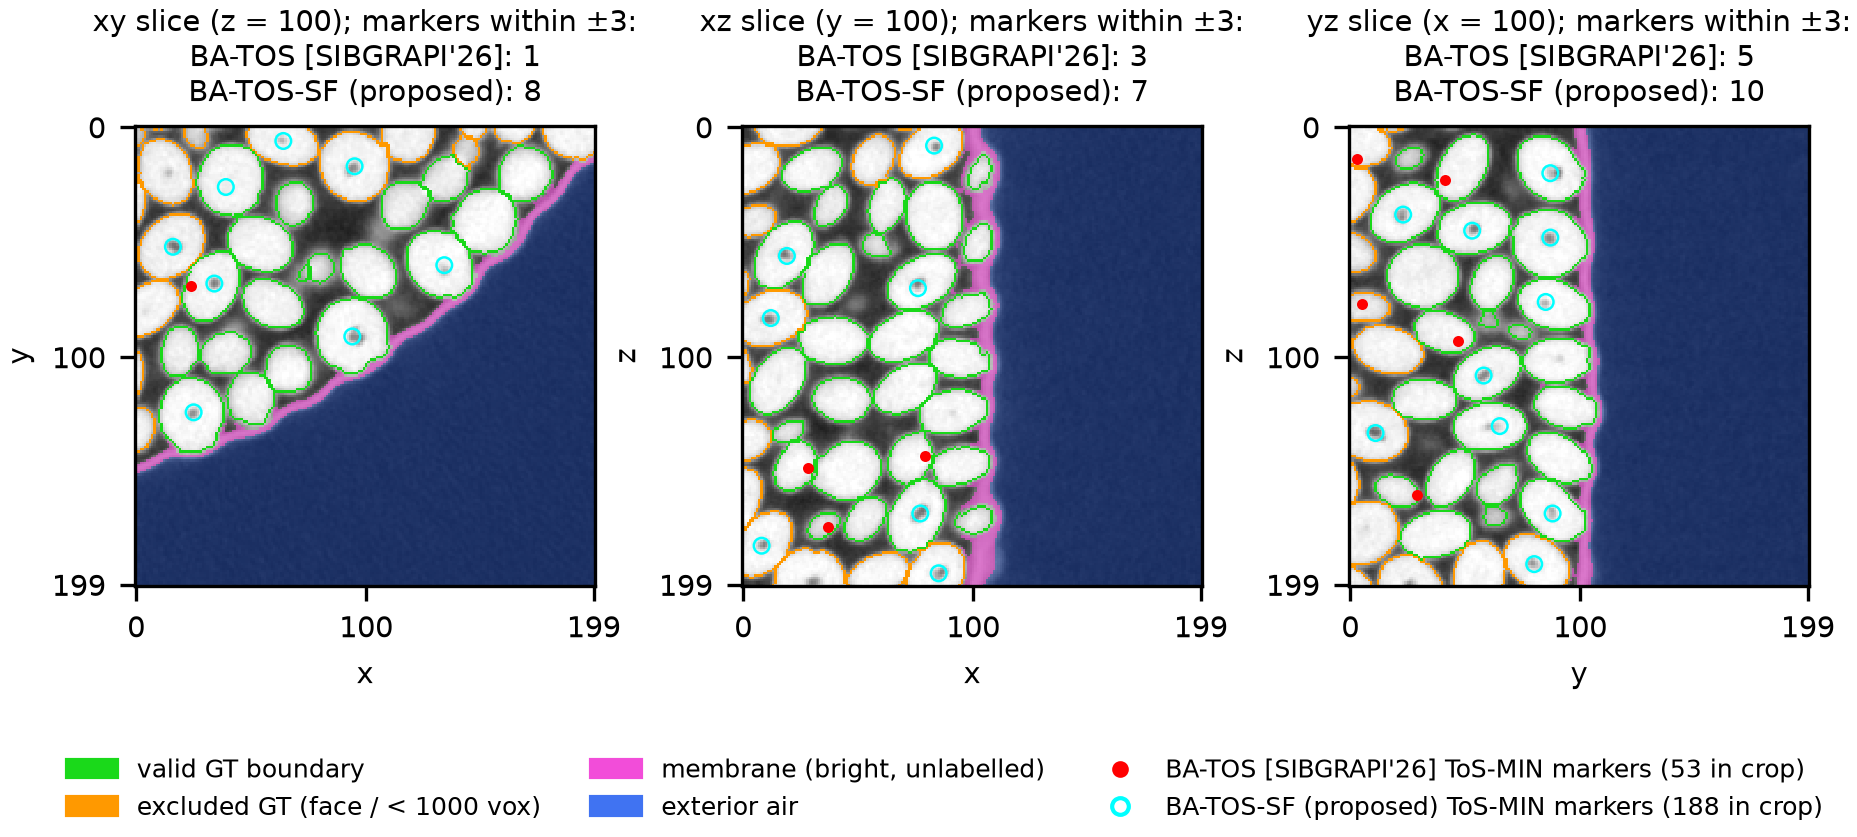
\includegraphics[width=\linewidth,height=0.44\textheight,keepaspectratio]{fig2_crop05_orthogonal_markers.png}\\
{\scriptsize Membrane (magenta), exterior air (blue, 51\,\% of the crop); markers: SIBGRAPI (red) vs \SF{} (cyan)}
\column{0.42\textwidth}
\centering
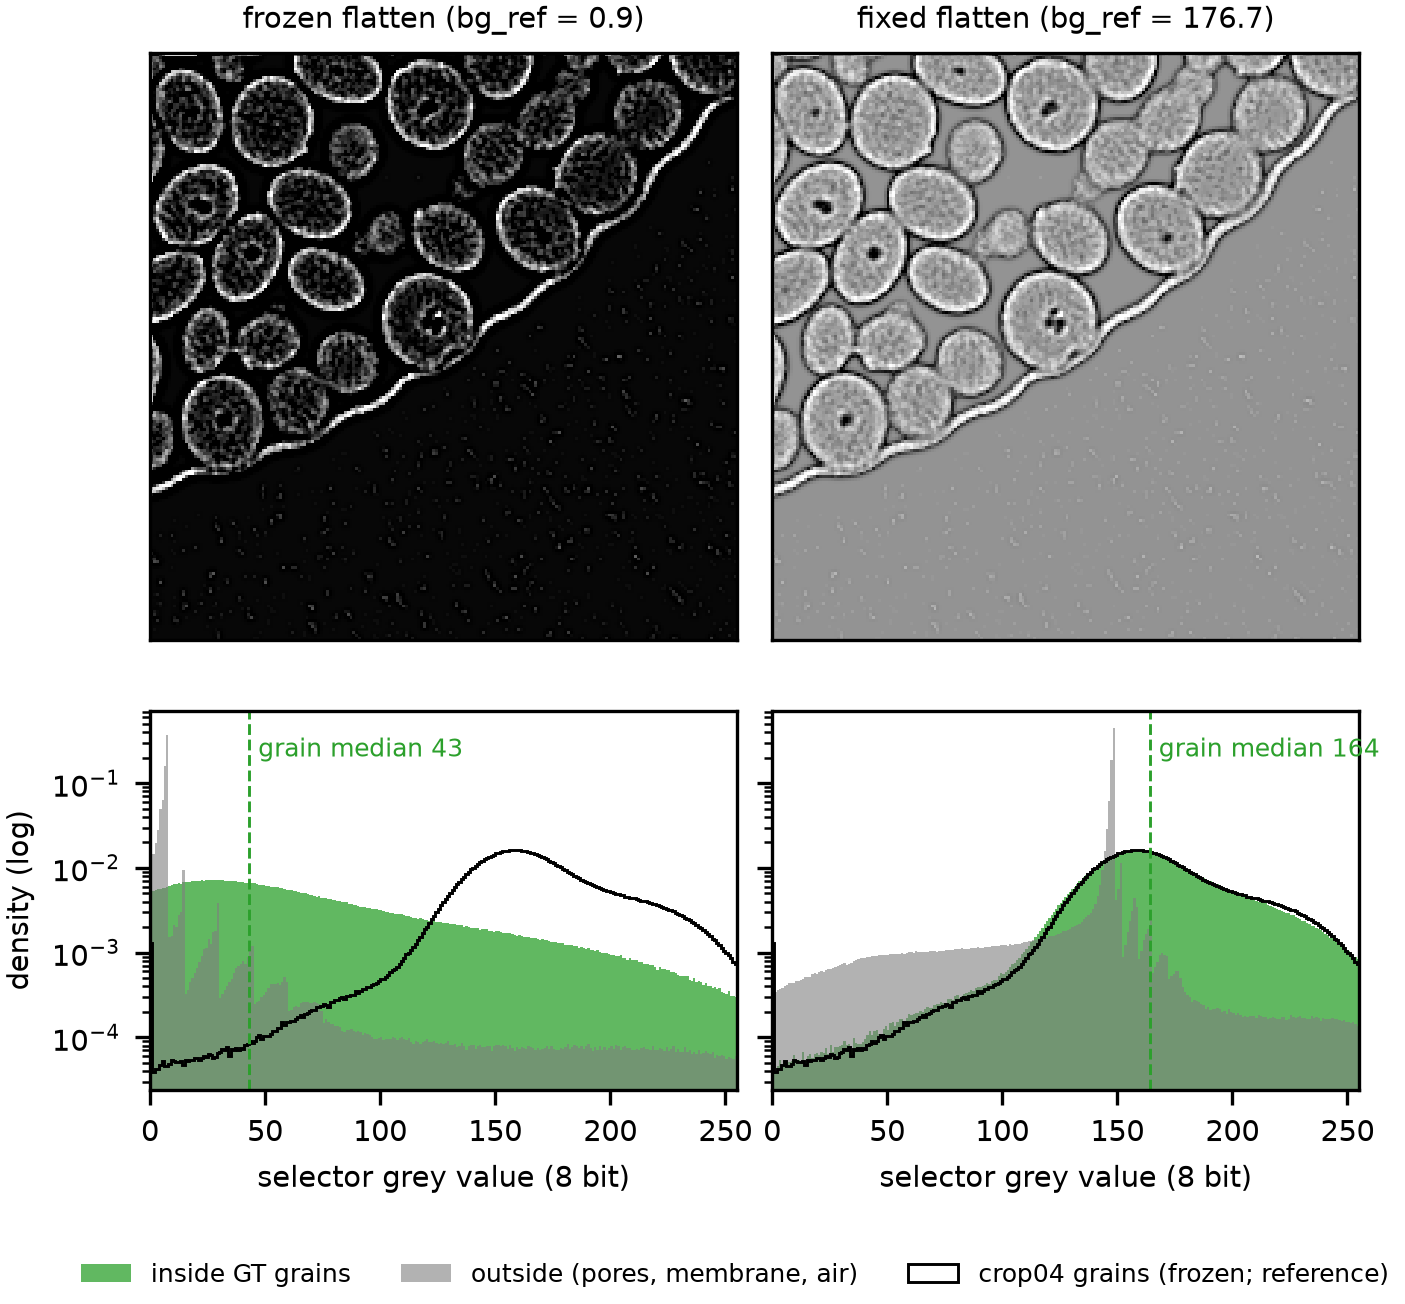
\includegraphics[width=\linewidth,height=0.48\textheight,keepaspectratio]{fig3_crop05_flatten_offset.png}\\
{\scriptsize Offset: 0.9 (whole crop) vs 176.7 (specimen only)}
\end{columns}

\vspace{0.25cm}
\begin{itemize}
  \item Air at value 0 drags $\mathrm{median}(blur>0)$ to 0.9; \textbf{one-line change:} $\mathrm{median}(blur \ge 1)$.
  \item With the offset computed on the specimen only, the collapse does not occur and the safeguard is no longer needed; crop-macro F1@0.50 \textbf{0.824 $\rightarrow$ 0.976}.
\end{itemize}
\end{frame}

% ---------------------------------------------------------------------------
% 4
\begin{frame}{Scale: a granulometric estimator with no parameter}
\centering
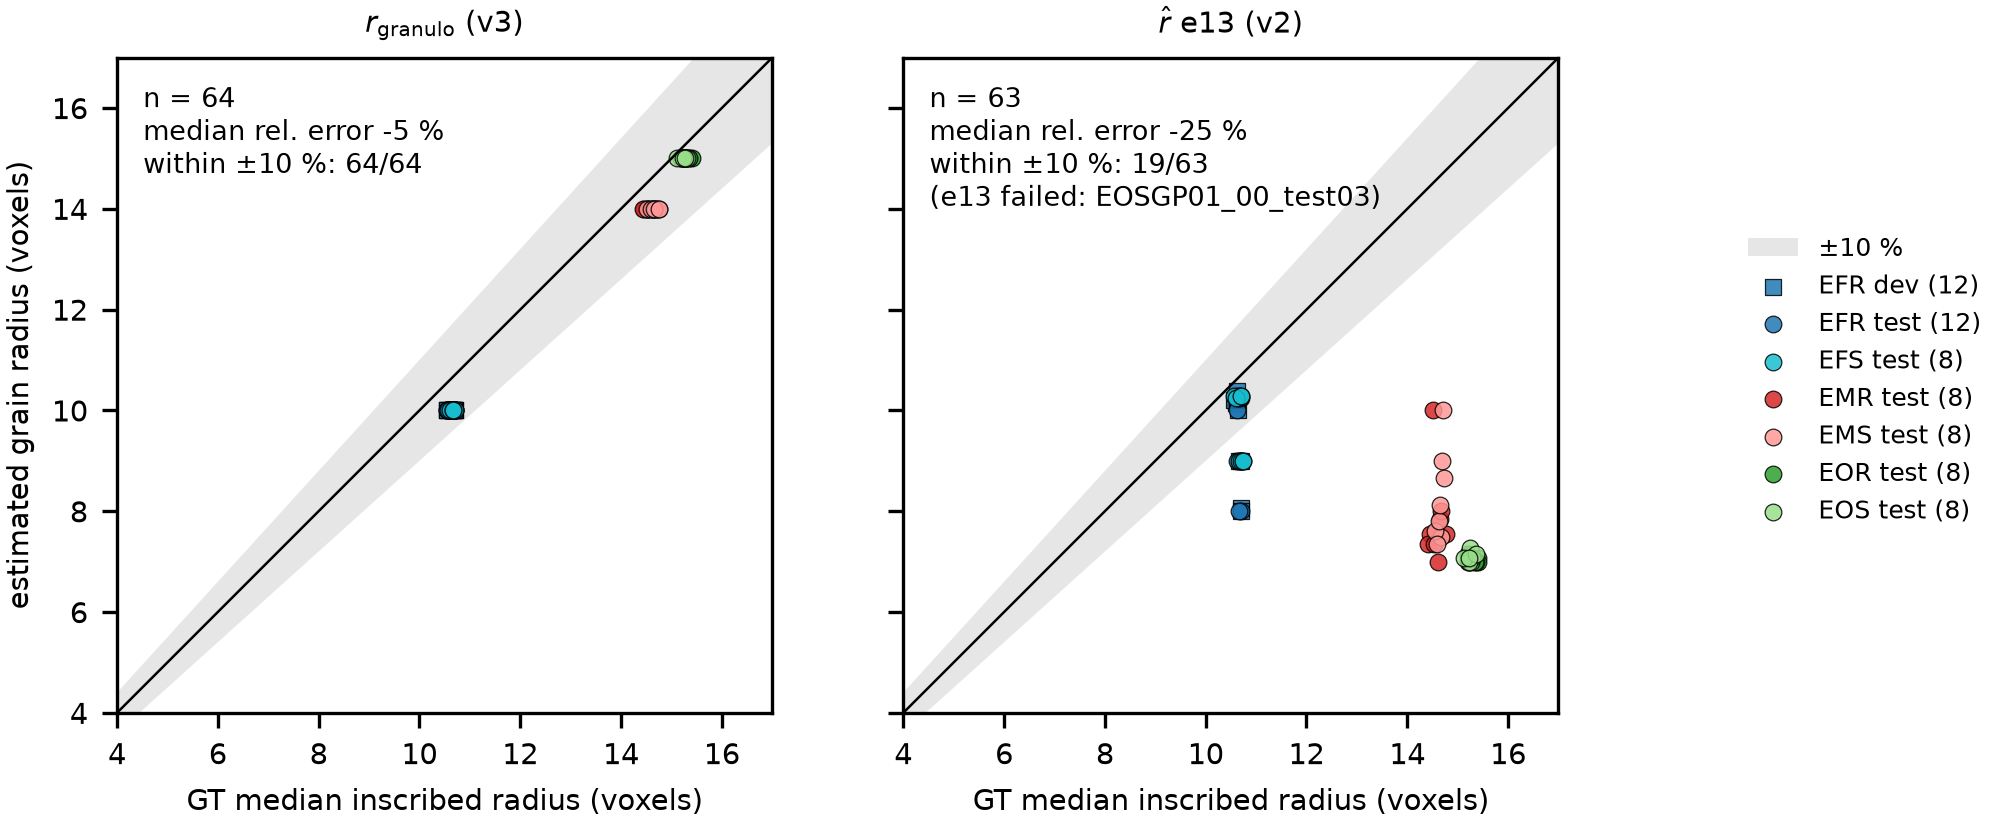
\includegraphics[width=\linewidth,height=0.58\textheight,keepaspectratio]{fig4_scale_estimates.png}

\vspace{0.15cm}
\raggedright
\begin{itemize}
  \item $r_\mathrm{granulo}$ = argmax of the pattern spectrum of the specimen foreground: \textbf{64/64 crops within $\pm$10\,\%} of the GT radius.
  \item The SIBGRAPI estimator (e13): 19/63 within $\pm$10\,\%; it \textbf{halves the radius} on the larger EM / EO grains.
\end{itemize}
\end{frame}

% ---------------------------------------------------------------------------
% 5
\begin{frame}{\SF{} (v3): what changed}
\begin{columns}[T,onlytextwidth]
\column{0.38\textwidth}
\begin{itemize}
  \item Scale from $r_\mathrm{granulo}$; every size constant follows $s = r_\mathrm{granulo}/10$.
  \item Thresholds from specimen-only statistics (Otsu inside the specimen).
  \item Absolute grey-level guards removed.
  \item Safeguard no longer needed (never activates on 52 test crops).
\end{itemize}
\column{0.60\textwidth}
\centering
\footnotesize
\begin{tabular}{lcc}
\toprule
\textbf{93 constants} & \textbf{SIBGRAPI} & \textbf{\SF} \\
\midrule
Fixed in voxels (size, volume, count) & 43 & \textbf{0} \\
Ad-hoc thresholds & 6 & \textbf{0} \\
Absolute grey-level guards & 3 & \textbf{0} \\
Dimensionless (kept) & 41 & 41 \\
\midrule
Safeguard activates (52 test crops) & 30 & \textbf{0} \\
\bottomrule
\end{tabular}

\vspace{0.1cm}
{\scriptsize Size constants scale as $s$, $s^3$ or $1/s^3$; on the dev crops $s=1$.}
\end{columns}
\src{docs/V3\_SCALE\_FREE.md (full constant table); paper/tables/test\_v3\_tables.tex}
\end{frame}

% ---------------------------------------------------------------------------
% 6
\begin{frame}{Held-out validation: 52 crops, 6 specimens}
\centering
\begin{adjustbox}{max width=0.88\linewidth,max totalheight=0.52\textheight}
\begin{tabular}{lrcccc}
\toprule
Specimen & $n$ & $\hat r$ / $r_\mathrm{in}$ & SIBGRAPI'26 & + specimen-only offset & \SF{} \\
\midrule
EFR & 12 & 10 / 10.6 & $0.879 \pm 0.223$ & $0.956 \pm 0.048$ & $\mathbf{0.985 \pm 0.011}$ \\
EFS &  8 & 10 / 10.6 & $0.882 \pm 0.155$ & $0.968 \pm 0.043$ & $\mathbf{0.974 \pm 0.044}$ \\
EMR &  8 & 14 / 14.5 & $0.303 \pm 0.439$ & $0.250 \pm 0.416$ & $\mathbf{0.980 \pm 0.027}$ \\
EMS &  8 & 14 / 14.7 & $0.432 \pm 0.465$ & $0.479 \pm 0.474$ & $\mathbf{0.986 \pm 0.020}$ \\
EOR &  8 & 15 / 15.3 & $0.293 \pm 0.362$ & $0.238 \pm 0.434$ & $\mathbf{0.754 \pm 0.240}$ \\
EOS &  8 & 15 / 15.3 & $0.265 \pm 0.429$ & $0.365 \pm 0.499$ & $\mathbf{0.754 \pm 0.214}$ \\
\midrule
External (5 spec.) & 40 & -- & $0.435 \pm 0.435$ & $0.460 \pm 0.473$ & $\mathbf{0.890 \pm 0.178}$ \\
All                & 52 & -- & $0.538 \pm 0.437$ & $0.575 \pm 0.465$ & $\mathbf{0.912 \pm 0.161}$ \\
\bottomrule
\end{tabular}
\end{adjustbox}

\vspace{0.2cm}
\raggedright
\begin{itemize}
  \item Protocol pre-registered: crop list committed before cutting (GT-free rule, fixed seed); nothing tuned on test.
  \item \SF{} reaches 0.98 on the EM specimens; 0.75 on the large-grained EO specimens.
\end{itemize}
{\tiny\color{gray}Crop-macro F1@0.50, seed-ignore, no size filter. Source: \texttt{results/test\_v3/}}
\end{frame}

% ---------------------------------------------------------------------------
% 7
\begin{frame}{Qualitative: 4 crops $\times$ 6 columns}
\centering
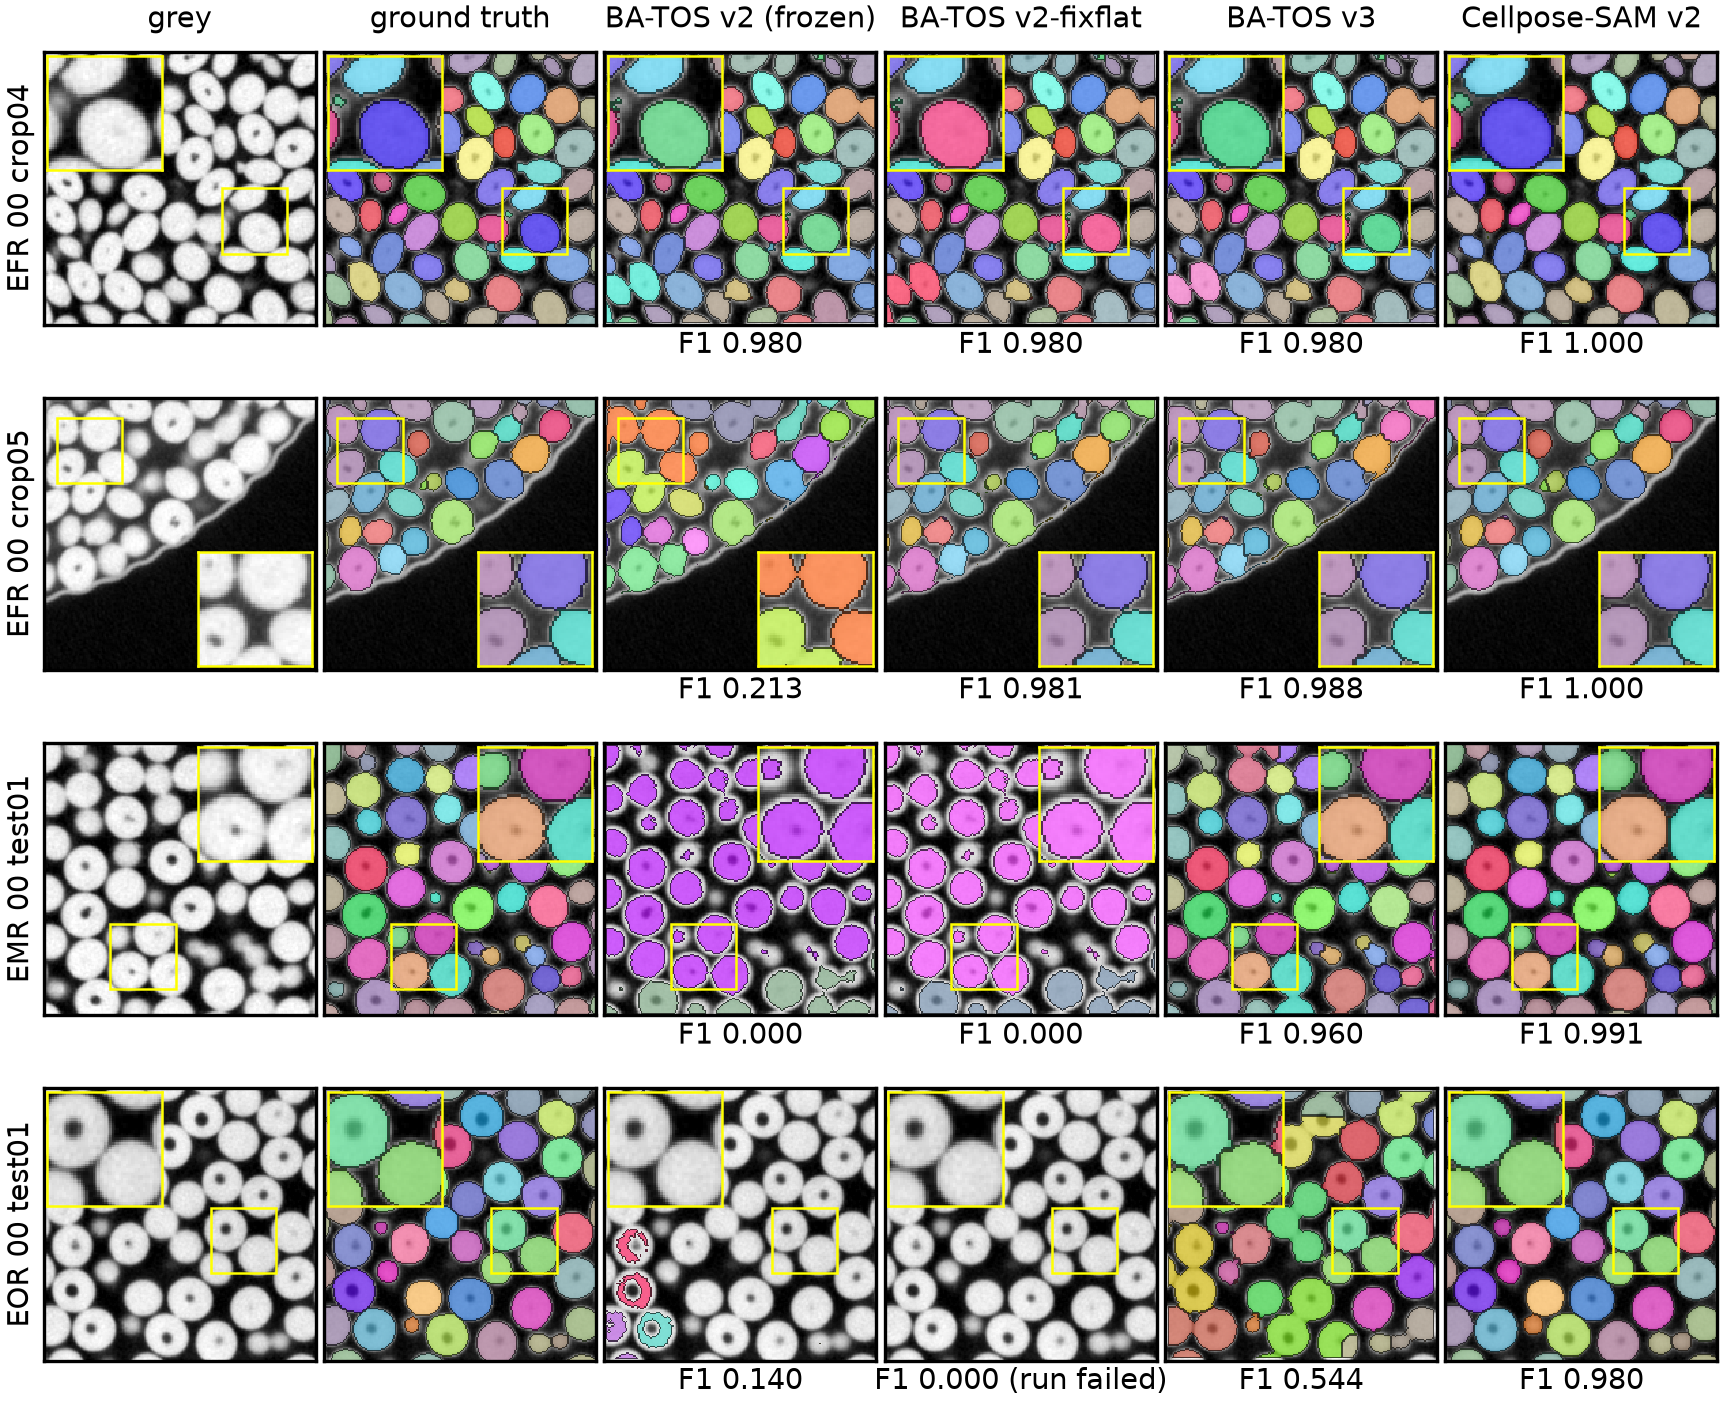
\includegraphics[width=\linewidth,height=0.86\textheight,keepaspectratio]{fig1_qualitative_slices.png}
\end{frame}

% ---------------------------------------------------------------------------
% 8
\begin{frame}{Parameter audit: 96 constants, 25 influential}
\begin{columns}[c,onlytextwidth]
\column{0.38\textwidth}
\begin{itemize}
  \item 96 method constants swept one at a time (12 dev crops); \textbf{25} move F1 by $>0.01$.
  \item Selector weights sit on a \textbf{narrow ridge}: halving or doubling one drops F1 by 0.4--0.6.
  \item \texttt{w\_support} has \textbf{no effect}: $\Delta = 0.000$.
\end{itemize}
\column{0.60\textwidth}
\centering
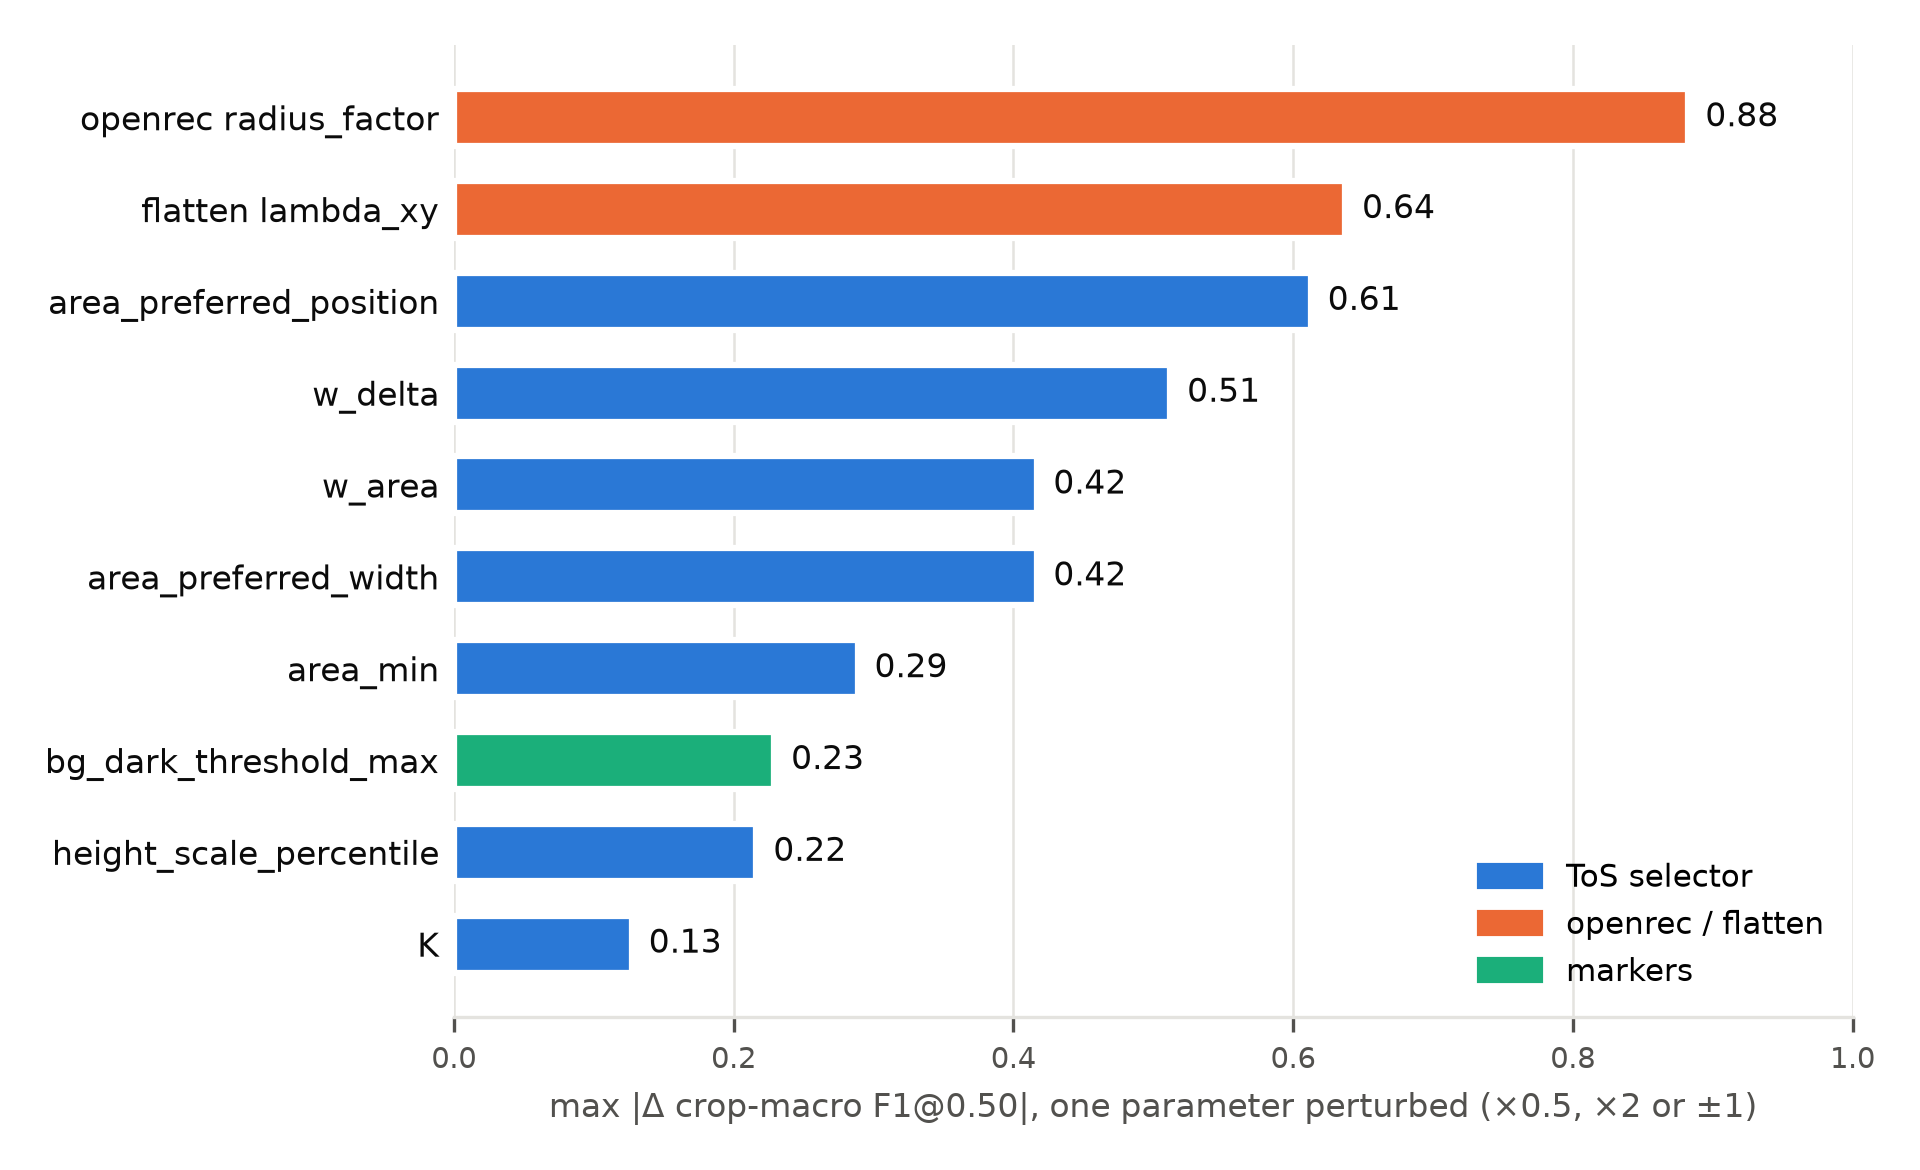
\includegraphics[width=\linewidth,height=0.78\textheight,keepaspectratio]{sens_top10.png}
\end{columns}
\src{results/sensitivity/ranking.csv (top 10 method parameters, BA-TOS\_sel route)}
\end{frame}

% ---------------------------------------------------------------------------
% 9
\begin{frame}{Comparison with Cellpose-SAM (default settings)}
\begin{columns}[T,onlytextwidth]
\column{0.40\textwidth}
\centering
\footnotesize
\begin{tabular}{lcc}
\toprule
Specimen & \texttt{cpsam\_v2} & \SF{} \\
\midrule
EFR & \textbf{0.999} & 0.977 \\
EFS & \textbf{0.999} & 0.964 \\
EMR & \textbf{0.998} & 0.966 \\
EMS & \textbf{0.999} & 0.970 \\
EOR & \textbf{0.996} & 0.735 \\
EOS & \textbf{0.998} & 0.727 \\
\midrule
All 52 & \textbf{0.998} & 0.896 \\
\bottomrule
\end{tabular}

\vspace{0.15cm}
\begin{tabular}{lcc}
\toprule
52 test crops & F1@0.50 & mIoU \\
\midrule
Cellpose-SAM & 0.998 & 0.899 \\
Cellpose, eroded 1 voxel & \textbf{0.999} & 0.917 \\
Hybrid & 0.996 & \textbf{0.923} \\
\bottomrule
\end{tabular}

{\tiny Crop-macro F1@0.50, no-marker evaluation (same rule for all).\\ Hybrid = Cellpose markers + \SF{} watershed.}
\column{0.57\textwidth}
\small
\begin{itemize}
  \item \textbf{Settings:} one default config, no fine-tuning; all four Cellpose 4 models agree within 0.002.
  \item \textbf{Robustness:} at 5\,\% added noise \SF{} drops to 0.13 / 0.06 / 0.00 (3 crops), \texttt{cpsam\_v2} $\ge 0.977$; at $2\times$ scale 0.963 vs 0.900.
  \item \textbf{Training data:} documented set = 19 cell/nuclei datasets, 2D (plus 98 natural photos); no micro-CT, granular data or Zenodo 8014905. The undocumented June 2026 models score the same as the documented \texttt{cpsam}.
  \item \textbf{Boundaries:} a 1-voxel erosion of Cellpose-SAM gives mIoU 0.917; the hybrid gives 0.923.
\end{itemize}
\end{columns}
\end{frame}

% ---------------------------------------------------------------------------
% Backup
\appendix
\begin{frame}{Backup: full-volume tiled \SF{}}
\centering
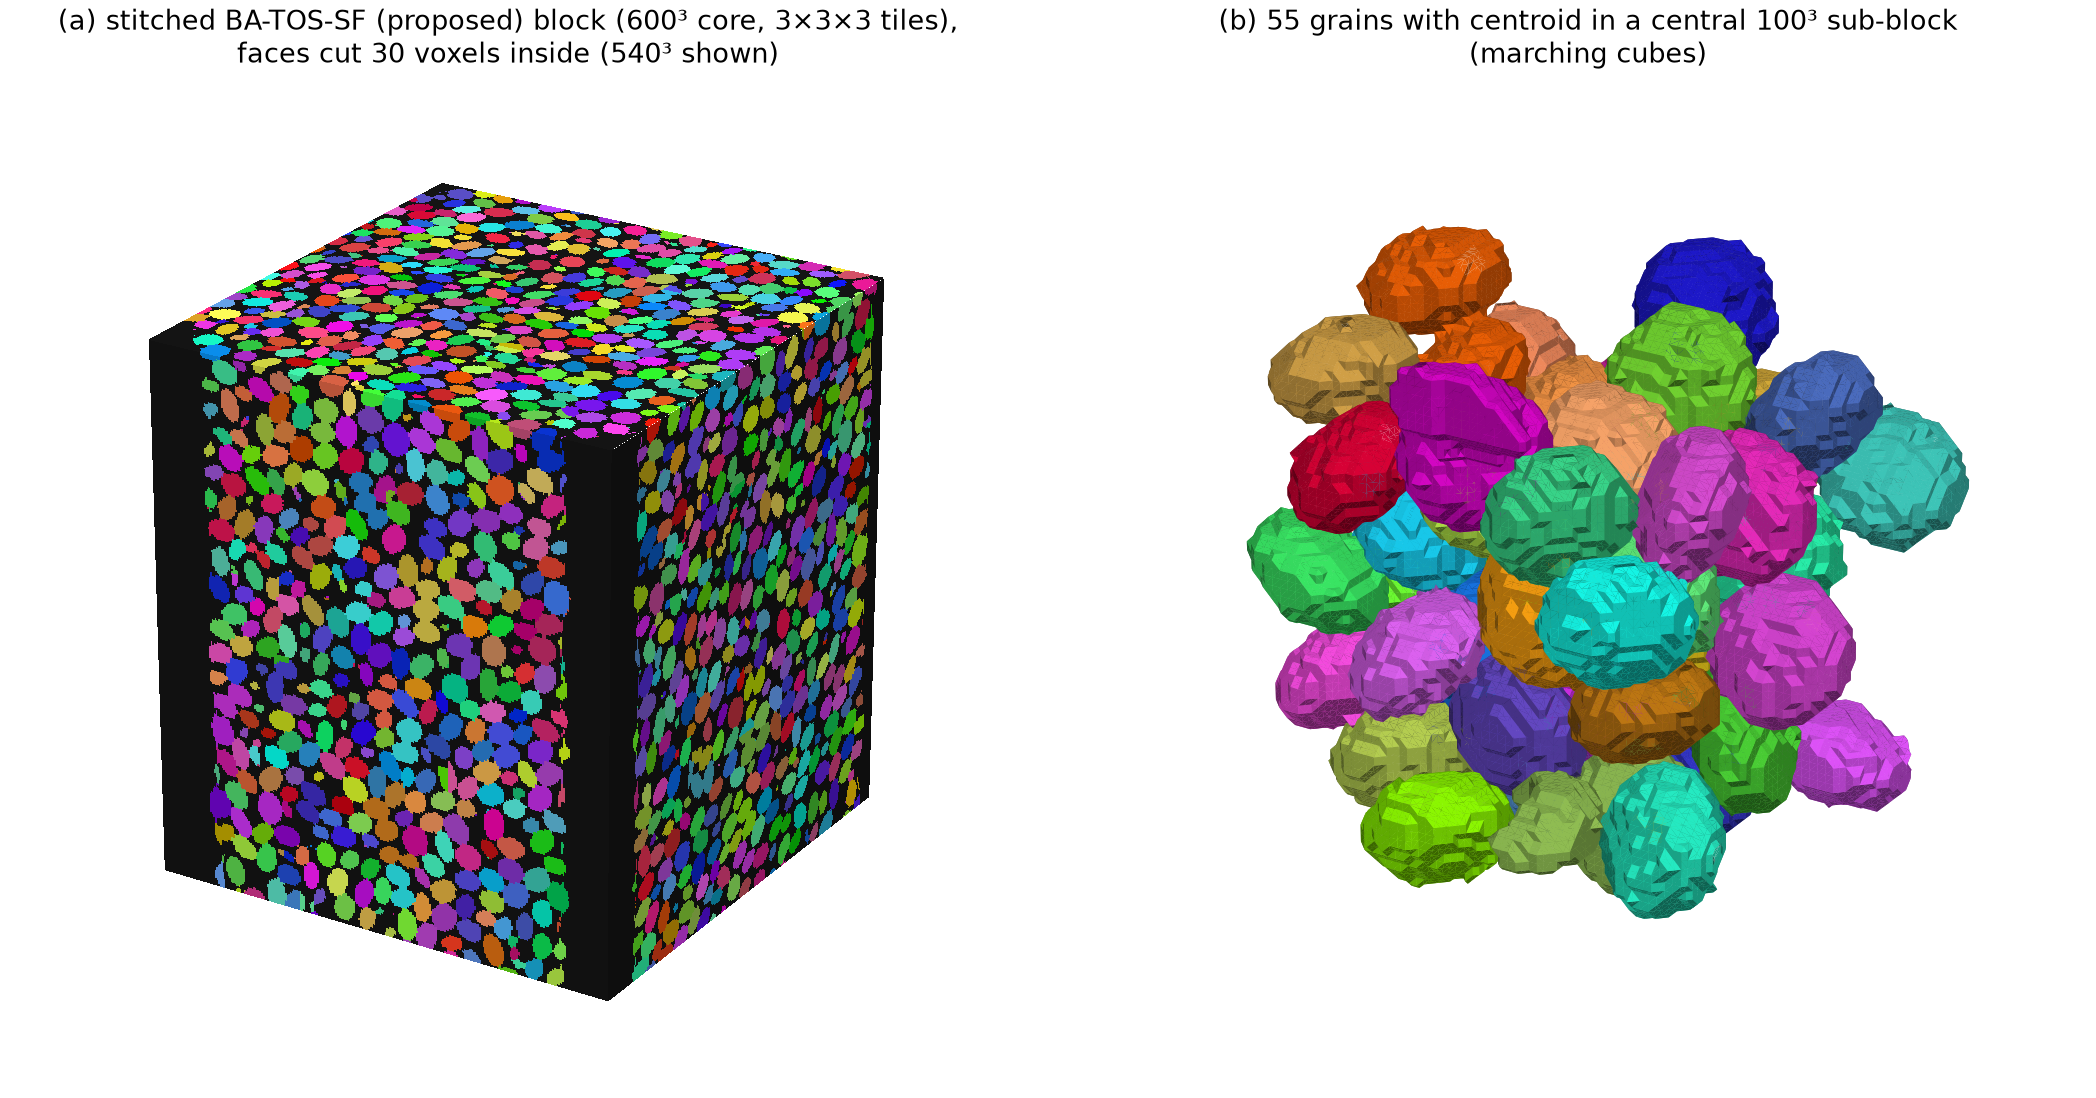
\includegraphics[width=\linewidth,height=0.66\textheight,keepaspectratio]{fig6_smoke_block_3d.png}

\raggedright
\begin{itemize}
  \item Central $3\times3\times3$ tiles of EFRGP01\_00: $600^3$ core, halo 20, orphan-rescue stitching.
  \item 9,753 instances; F1@0.50 = 0.865 on the 6,005 valid GT grains (seed-ignore, no filter).
\end{itemize}
\end{frame}

\end{document}
